\begin{exercise}{Photo aillée}{2}{Sup}
{Interference, Michelson}{lelay, centrale}

Une tête d'ail fait à peu près 7 cm de diamètre. Cette photo a été prise à une distance $D$ de l'ail avec un appareil de distance focale $f' = 50$ mm en utilisant un diaphragme de rayon $R$ et une pellicule de 24x36 mm placée à une distance $d$ de la lentille.

\begin{figure}[H]
    \centering
    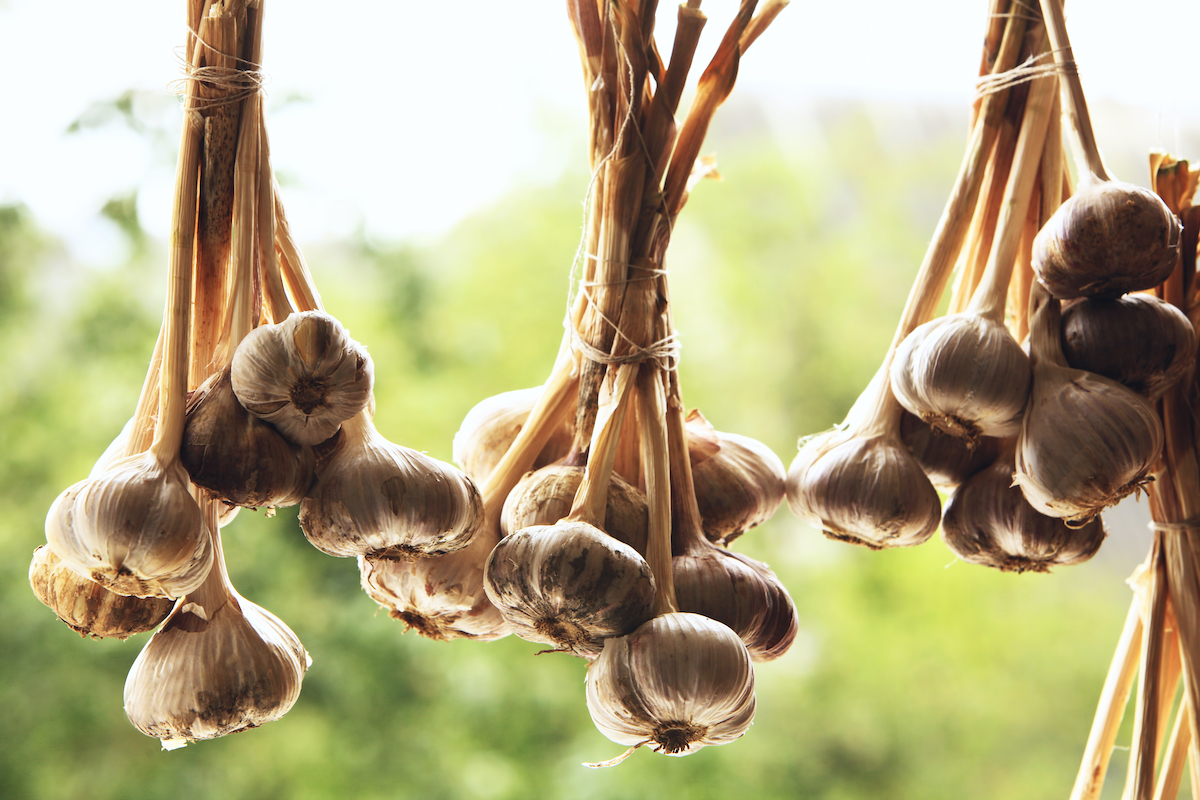
\includegraphics[width=.8\linewidth]{optique/optiquegeometrique/ail.jpg}
    \caption{Ail.}
\end{figure}

\begin{questions}
    \questioncours Lentilles convergentes, relations de conjugaisons.
    \question Déterminer la taille des gousses d’ail sur la pellicule. En déduire $d$ et $D$.
    \question On voit sur la photos des ronds clairs qui viennent d’objets au loin. Déterminer leur taille sur la pellicule, en déduire le rayon
du diaphragme $R$. Donner le nombre d'ouverture de l'appareil $\frac{f'}{2R}$.
    \question À quel phénomène aurait-on pu penser pour expliquer ronds ? Montrer quantitativement que ce n’est pas dû à cette cause.
    \question Quelle semble être la distance maximale jusqu’à laquelle on voit net ? En déduire la taille d’un élément photosensible sur cette
pellicule. Comparer à la résolution en pixels d’un appareil récent.
\end{questions}

\end{exercise}

\begin{solution}
\begin{questions}
    \questioncours $1/D+1/d=1/f'$ (Descartes)
    \question Avec un schéma et Thalès on trouve que $\frac{d}{D} ={5\text{ mm}}{7\text{ cm}}$ soit $D=75$ cm et $d=54$ mm.
    \question On prend un rayon qui vient de l’infini, si on appelle $\delta$ la taille d'un rond sur la pellicule ($\sim 1.7$ mm) alors par Thalès $\frac{\delta/2}{R}=\frac{d-f'}{f'}$ on trouve $R$ de l'ordre de $1$ cm.
    \question La diffraction. OdG de diffraction, on a $\lambda \ll R$ donc c'est mort.
    \question On voit net sur a peu pres 1 tête soit une profondeur de champ d'une dizaine de cm. Un objet situé à $D-5$ cm serait nette dans le plan situé à $d+\delta d = 57$ mm. Thalès ensuite avec les deux plus grands rayons venant de cet objet sur l'axe optique donne $\frac{\epsilon}{R} = \frac{\delta d}{d+\delta d}$ soit ici a peu près 0.5 mm. On trouve un elment photosensible de 0.1 mm$^2$ ce qui est grand devant la taille en pixel des caméras récentes.
\end{questions}
\end{solution}